\documentclass[11pt]{article}

\usepackage[margin=1in]{geometry}
\usepackage[T1]{fontenc}
\usepackage{lmodern}
\usepackage{microtype}
\usepackage{amsmath,amssymb}
\usepackage{booktabs}
\usepackage{graphicx}
\usepackage{xcolor}
\usepackage[numbers,sort&compress]{natbib}
\usepackage{tikz}
\usetikzlibrary{positioning,arrows.meta,fit,calc}
\usepackage[colorlinks=true,linkcolor=blue!60!black,citecolor=blue!60!black,urlcolor=blue!60!black]{hyperref}
\usepackage{cleveref}

\newcommand{\tok}[1]{\texttt{<#1>}}

\title{\textbf{HALE-WAM: A Compact World--Action Model that Perceives, Reasons,\\Acts and Imagines in One Transformer}}
\author{B A NaveenKumar\\
\small Independent researcher\\
\small \url{https://github.com/basaanithanaveenkumar/HALE-WAM}}
\date{}

\begin{document}
\maketitle

\begin{abstract}
Robot policies that can also \emph{predict the visual consequences} of their actions are
easier to inspect and can learn from video without action labels. We present
\textbf{HALE-WAM}, a 176M-parameter world--action model that, from a few camera frames, a
proprioceptive state and a language instruction, jointly (i)~generates a text response,
(ii)~samples a continuous action chunk with a conditional flow-matching head, and
(iii)~imagines future RGB frames with a Diffusion Transformer (DiT). All three outputs are
read from a single causal mixture-of-experts transformer through special tokens:
\tok{halo\_action} hidden states condition the action velocity field, and
\tok{halo\_world\_video} hidden states act as per-frame queries for the world model. Each
predicted frame receives its own conditioning vector, built from a cross-attended query, a
sinusoidal frame-index embedding, a pixel encoding of the last observed frame and a learned
null token for classifier-free guidance. This vector modulates the DiT through a gated
adaLN-Zero pathway. Frames are sampled with Heun's second-order ODE solver, and training
adds VGG-perceptual, SSIM and temporal-smoothness losses on the implied clean-frame
estimate to reduce blur. We describe the architecture, the joint objective and the
training infrastructure (mixed precision, gradient accumulation, gradient checkpointing,
resumable checkpoints), and show qualitative results on AIRoA MoMa mobile-manipulation
episodes.
\end{abstract}

\section{Introduction}

Vision--language--action (VLA) models~\cite{brohan2023rt2,kim2024openvla,black2024pi0} map
observations and instructions to actions, but give little insight into \emph{why} a given
action was chosen. World models~\cite{ha2018worldmodels,hafner2023dreamerv3} learn to predict
how observations evolve, and recent robot-learning work uses video generation as a policy
prior~\cite{du2023unipi,wu2023gr1}. Combining the two in one network is attractive. The
imagined future is a directly inspectable explanation of the plan, and the video-prediction
objective provides dense supervision even where action labels are missing or noisy.

HALE-WAM is a compact, from-scratch implementation of this idea. Its design goals are
(1)~one shared backbone for language, action and imagination, (2)~continuous and multi-modal
action distributions, and (3)~sharp, frame-specific future predictions at small scale.
Our contributions are:
\begin{itemize}
  \item A \textbf{four-token interface} (\tok{image}, \tok{state}, \tok{halo\_action},
        \tok{halo\_world\_video}) that routes one causal MoE decoder to three output heads
        (\cref{sec:backbone}).
  \item A \textbf{flow-matching action head} conditioned on \tok{halo\_action} hidden
        states that predicts 16-step action chunks by integrating a learned velocity field
        (\cref{sec:flow}).
  \item A \textbf{per-frame conditioned DiT world model} with four stacked conditioning
        signals, gated adaLN-Zero fusion, classifier-free guidance and a Heun sampler
        (\cref{sec:dit}).
  \item \textbf{Anti-blur auxiliary losses} computed on the analytic clean-frame estimate
        $\hat x_1=x_t+(1-t)\,v_\theta$ (\cref{sec:losses}).
\end{itemize}

\section{Related Work}

\paragraph{VLAs and action heads.} RT-2~\cite{brohan2023rt2} and
OpenVLA~\cite{kim2024openvla} emit discretised action tokens. Octo~\cite{octo2024} uses a
diffusion head and $\pi_0$~\cite{black2024pi0} a flow-matching action expert. ACT~\cite{zhao2023aloha}
predicts action chunks. HALE-WAM follows $\pi_0$ in using flow matching over action chunks
but keeps the velocity network small and conditions it on a single decoder hidden state.

\paragraph{Flow matching and diffusion transformers.} Conditional flow
matching~\cite{lipman2023flow} and rectified flow~\cite{liu2023rectified} learn straight-line
probability paths between noise and data, and allow few-step deterministic sampling.
DiT~\cite{peebles2023dit} replaces the U-Net with a transformer modulated by adaptive
LayerNorm. Classifier-free guidance~\cite{ho2022cfg} trades diversity for fidelity, and
second-order Heun integration~\cite{karras2022edm} reduces discretisation error.

\paragraph{World models for robotics.} UniPi~\cite{du2023unipi} plans by generating videos
and inverting them to actions. GR-1~\cite{wu2023gr1} pretrains a GPT-style model on video
prediction before fine-tuning for manipulation. Stable Video Diffusion~\cite{blattmann2023svd}
conditions generation on a context frame, which inspires our pixel-level anchor. HALE-WAM
trains action prediction and video prediction jointly from the same hidden states.

\section{Method}

\begin{figure}[t]
\centering
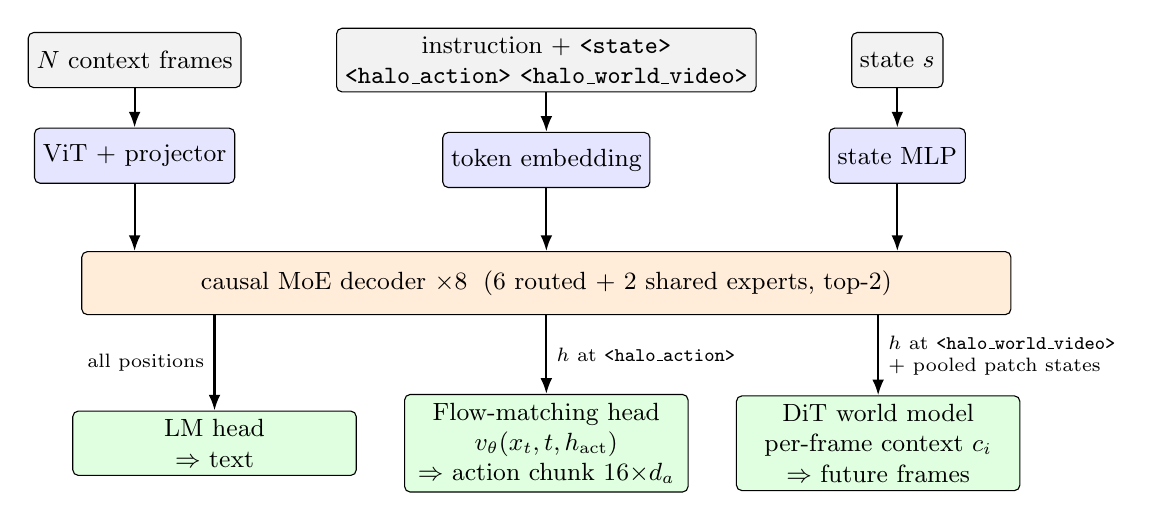
\begin{tikzpicture}[
  node distance=5mm and 5mm,
  box/.style={draw, rounded corners=2pt, align=center, font=\small, minimum height=7mm, inner sep=3pt},
  inp/.style={box, fill=gray!10},
  enc/.style={box, fill=blue!10},
  core/.style={box, fill=orange!15, minimum width=118mm, minimum height=8mm},
  head/.style={box, fill=green!12, minimum width=36mm},
  arr/.style={-{Latex[length=2mm]}, thick}
]
\node[inp] (img) {$N$ context frames};
\node[inp, right=12mm of img] (txt) {instruction + \tok{state}\\\tok{halo\_action} \tok{halo\_world\_video}};
\node[inp, right=12mm of txt] (st) {state $s$};
\node[enc, below=of img] (vit) {ViT + projector};
\node[enc, below=of txt] (emb) {token embedding};
\node[enc, below=of st] (senc) {state MLP};
\node[core, below=8mm of emb] (dec) {causal MoE decoder $\times 8$ \;(6 routed + 2 shared experts, top-2)};
\draw[arr] (img) -- (vit); \draw[arr] (txt) -- (emb); \draw[arr] (st) -- (senc);
\draw[arr] (vit) -- (vit |- dec.north); \draw[arr] (emb) -- (dec); \draw[arr] (senc) -- (senc |- dec.north);
\node[head, below=10mm of dec] (fm) {Flow-matching head\\$v_\theta(x_t,t,h_{\text{act}})$\\$\Rightarrow$ action chunk $16{\times}d_a$};
\node[head, left=6mm of fm] (lm) {LM head\\$\Rightarrow$ text};
\node[head, right=6mm of fm] (dit) {DiT world model\\per-frame context $c_i$\\$\Rightarrow$ future frames};
\draw[arr] (dec.south -| lm) -- node[left, font=\scriptsize]{all positions} (lm);
\draw[arr] (dec) -- node[right, font=\scriptsize]{$h$ at \tok{halo\_action}} (fm);
\draw[arr] (dec.south -| dit) -- node[right, font=\scriptsize, align=left]{$h$ at \tok{halo\_world\_video}\\+ pooled patch states} (dit);
\end{tikzpicture}
\caption{HALE-WAM overview. One decoder is read by three heads: the LM head at every
position, the flow-matching action head at \tok{halo\_action} positions, and the DiT world
model at \tok{halo\_world\_video} positions.}
\label{fig:arch}
\end{figure}

\subsection{Shared backbone}
\label{sec:backbone}

Text is tokenised with the 49{,}152-token cosmo2 tokenizer used by SmolLM~\cite{allal2025smollm2},
which follows the ChatML format but is about $3\times$ smaller than Qwen's vocabulary. Four
special tokens extend it to $V=49{,}156$. Each $224\times224$ context frame is encoded by a
dense six-layer ViT~\cite{dosovitskiy2021vit} (patch size 16, 196 patches) and a
three-layer MLP projector, and the patches of all frames are prepended to the text. State
vectors are encoded by an MLP and written in place of their \tok{state} tokens. A learned
absolute position embedding is added to the combined sequence, which is processed by
8 pre-LN causal transformer blocks ($d=512$, 16 heads) whose feed-forward layers are
DeepSeekMoE~\cite{dai2024deepseekmoe} layers with 2 shared and 6 routed SwiGLU~\cite{shazeer2020glu}
experts (noisy top-2 routing~\cite{shazeer2017outrageously}). Unlike Hale-VLA,
the decoder applies a key-padding mask built from the text attention mask (image patches are
always valid) and uses gradient checkpointing~\cite{chen2016checkpointing} to fit long
multi-frame sequences in memory.

The decoder output feeds three heads. The \textbf{LM head} predicts next tokens at every
position. The hidden states at \tok{halo\_action} positions, $h_{\text{act}}$, condition the
\textbf{action head}. The hidden states at \tok{halo\_world\_video} positions,
$h_{\text{wv},i}$, together with a visual context vector $\bar h_{\text{vis}}$, condition
the \textbf{world model}. $\bar h_{\text{vis}}$ is the mean of the decoder outputs at the
patch positions of each frame, averaged over all frames strictly before the last valid one.

\subsection{Flow-matching action head}
\label{sec:flow}

Let $x_1\in\mathbb{R}^{C d_a}$ be a flattened ground-truth action chunk ($C=16$ steps) and
$x_0\sim\mathcal N(0,I)$. Following conditional flow matching with the optimal-transport
path~\cite{lipman2023flow,liu2023rectified},
\begin{equation}
  x_t=(1-t)\,x_0+t\,x_1,\qquad t\sim\mathcal U(0,1),\qquad
  \mathcal L_{\text{act}}=\big\lVert v_\theta(x_t,t,h_{\text{act}})-(x_1-x_0)\big\rVert_2^2 .
\end{equation}
$v_\theta$ is a four-layer MLP (width 1024, ReLU) applied to the concatenation of $x_t$, a
128-dimensional sinusoidal embedding of $t$, and $h_{\text{act}}$. At inference we
integrate $\dot x=v_\theta(x,t,h_{\text{act}})$ from $t=0$ to $1$ with 24 Euler steps.
Unlike a regression head, this can represent multi-modal action distributions.

\subsection{DiT world model}
\label{sec:dit}

\paragraph{Denoiser.} Future frames are generated in pixel space by a DiT~\cite{peebles2023dit}
with patch size 8 (784 tokens at $224\times224$), hidden size 512, depth 8 and 8 heads.
Every block uses adaLN-Zero modulation (shift, scale and gate for attention and MLP,
zero-initialised). The same flow-matching objective as the action head is used, with
$x_1$ a target frame.

\paragraph{Per-frame conditioning.} Frame $i$ (global index $f+i$) gets its own conditioning
vector $c_i$, built from four stacked signals:
\begin{align}
  q_i &= \begin{cases} W_q\,h_{\text{wv},i} & \text{if a \tok{halo\_world\_video} token is present}\\ w_{f+i} & \text{otherwise (learned per-frame token)}\end{cases}\\
  b_i &= \mathrm{LN}\!\big(u_i + \mathrm{FFN}(u_i)\big),\quad u_i=\mathrm{LN}\big(q_i+\mathrm{CrossAttn}(q_i,\ \bar h_{\text{vis}})\big),\\
  c_i &= b_i + W_p\,\mathrm{PE}(f+i) + \mathrm{Drop}_{0.2}\big(E_{\text{pix}}(I_{\text{last}})\big).
\end{align}
The sinusoidal frame-index term $\mathrm{PE}$ makes frames distinguishable even when the
queries are similar. $E_{\text{pix}}$, two strided convolutions, global pooling and a linear
layer, encodes the last observed frame $I_{\text{last}}$ as a pixel-level scene anchor in
the spirit of Stable Video Diffusion~\cite{blattmann2023svd}. It is dropped out so the model
does not over-rely on perfect context frames. With probability 0.1 during training, $c_i$
is replaced by a learned null vector $c_\varnothing$ to enable classifier-free
guidance~\cite{ho2022cfg}.

\paragraph{Gated fusion.} Inside the DiT the conditioning multiplicatively gates the timestep
embedding rather than being added to it,
\begin{equation}
  \tilde c = \sigma(W_g c_i)\odot \mathrm{emb}(t) + W_c\,c_i ,
\end{equation}
and $\tilde c$ drives adaLN in every block. The gate bias is zero-initialised, so time and
context are blended equally at the start of training.

\paragraph{Sampling.} Frames are generated with Heun's second-order method~\cite{karras2022edm},
\begin{equation}
  \tilde x = x + \Delta t\, v_1,\quad x \leftarrow x + \tfrac{\Delta t}{2}\,(v_1+v_2),\quad
  v_1=\hat v(x,t),\ v_2=\hat v\big(\tilde x,\min(t{+}\Delta t,1{-}10^{-5})\big),
\end{equation}
with guided velocity $\hat v = v_\varnothing + w\,(v_c - v_\varnothing)$ when $w>1$. Longer
horizons are rolled out autoregressively: after each frame, the visual context is
re-encoded from the frames seen so far.

\subsection{Training objective}
\label{sec:losses}

Pure velocity MSE in pixel space produces blurry frames. Because the OT path gives an exact
estimate of the clean frame, $\hat x_1 = \mathrm{clip}_{[0,1]}\big(x_t+(1-t)\,v_\theta\big)$,
we add image-space losses on $\hat x_1$:
\begin{equation}
  \mathcal L_{\text{vis}} = \mathcal L_{\text{CFM}}
  + \lambda_{p}\,\mathcal L_{\text{VGG}}(\hat x_1,x_1)
  + \lambda_{s}\,\big(1-\mathrm{SSIM}(\hat x_1,x_1)\big)
  + \lambda_{\tau}\,\tfrac{1}{F-1}\textstyle\sum_i \lVert v_{i+1}-v_i\rVert_2^2 ,
\end{equation}
where $\mathcal L_{\text{VGG}}$ is a feature-space MSE at VGG-16~\cite{simonyan2015vgg}
relu1\_2 and relu2\_2~\cite{johnson2016perceptual}, SSIM uses an $11\times11$ Gaussian
window~\cite{wang2004ssim}, and the last term encourages temporally smooth velocity fields
across the $F$ predicted frames. The full objective is
\begin{equation}
  \mathcal L = \mathcal L_{\text{lang}} + \lambda_{a}\,\mathcal L_{\text{act}} + \lambda_{v}\,\mathcal L_{\text{vis}},
\end{equation}
with $\mathcal L_{\text{lang}}$ the next-token cross-entropy on assistant tokens (offset by
the prepended patches). The defaults are $\lambda_a=1$, $\lambda_v=8$, $\lambda_p=0.1$,
$\lambda_s=0.4$ and $\lambda_\tau=0.2$.

\section{Implementation}

\Cref{tab:params} gives the measured parameter budget of the default configuration. Training
uses AdamW~\cite{loshchilov2019adamw}, automatic mixed precision with a gradient scaler,
gradient accumulation (the loss is divided by the number of micro-steps so accumulated
gradients equal the large-batch average), gradient clipping at 1.0 and checkpoints that
restore model, optimiser, scheduler and scaler state. Data loaders support
EO-Data1.5M~\cite{qu2025eo1}, the AIRoA MoMa mobile-manipulation dataset~\cite{airoamoma}
(multi-frame clips with configurable stride, sampled as $N$ context frames plus $F$ future
frames) and DROID~\cite{khazatsky2024droid} in LeRobot format. The training script writes
GIFs that show the context frames, the generated answer, predicted versus ground-truth
action curves and predicted versus ground-truth future frames.

\begin{table}[t]
\centering
\caption{Parameter budget of the default HALE-WAM configuration (measured from the released code).}
\label{tab:params}
\begin{tabular}{lrl}
\toprule
Module & Parameters & Notes \\
\midrule
Vision encoder (ViT) & 10.0M & 6 dense layers, patch 16 \\
Image projector & 0.23M & $512\to128\to256\to512$ \\
Token embedding & 25.2M & $V=49{,}156$ \\
Position embedding & 1.0M & 2{,}000 positions \\
Decoder (MoE) & 68.8M & 8 layers, 6 routed / 2 shared experts, top-2 \\
LM head & 25.2M & \\
State encoder & 0.40M & \\
Flow-matching action head & 3.0M & 4-layer MLP, width 1024 \\
DiT world model & 42.5M & DiT 39.5M + conditioning 3.0M \\
\midrule
Total & 176.3M & \\
\bottomrule
\end{tabular}
\end{table}

\section{Qualitative Results}

\begin{figure}[t]
\centering
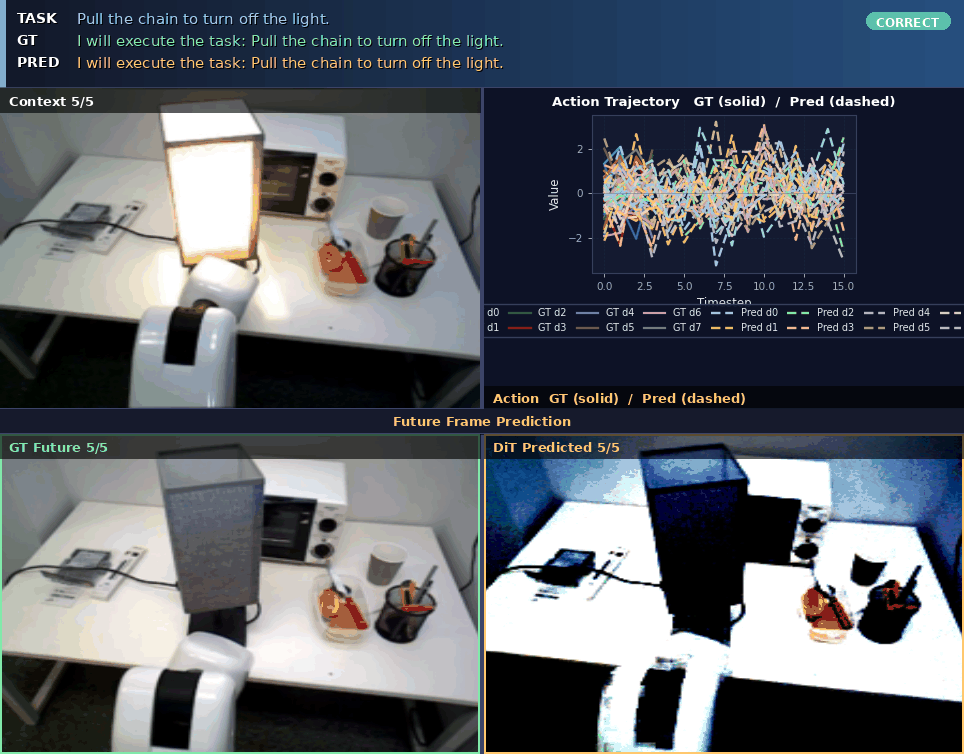
\includegraphics[width=0.92\linewidth]{figures/qualitative.png}
\caption{Output of the training visualiser at step 24{,}000 on an AIRoA MoMa episode
(``Pull the chain to turn off the light''). Top: the generated response matches the ground
truth. Right: predicted (dashed) versus ground-truth (solid) action dimensions over the
16-step chunk. Bottom: ground-truth versus DiT-predicted fifth future frame. The prediction
recovers the scene layout, the lamp being switched off and the gripper position, but shows
saturated contrast and blocky artefacts at the $8\times8$ patch scale.}
\label{fig:qual}
\end{figure}

\Cref{fig:qual} shows a sample produced during training. The language head reproduces the
target response, and the world model predicts the correct \emph{semantic} change: the lamp
turns dark after the chain is pulled. However, the predicted frame is over-contrasted and
shows patch-scale artefacts, which is typical of pixel-space DiTs at this size. The action
curves follow the overall range of the ground truth but not individual high-frequency
dimensions. We stress that this is a qualitative sample from a single run, not a benchmark
result.

% TODO: add quantitative results only once they are produced by scripts in this repo.
Quantitative evaluation is in progress. It covers action MSE and success-weighted metrics on
held-out MoMa episodes, PSNR/SSIM/LPIPS of predicted frames as a function of horizon, CFG
scale and number of Heun steps, and ablations of each conditioning signal in \cref{sec:dit}.

\section{Limitations and Future Work}

The DiT operates on raw pixels, which limits resolution and sharpness. A VAE latent space
(a \texttt{VideoVAE} module is included but not yet used in training) would reduce the
784-token sequence and improve fidelity. The action head samples with first-order Euler
steps and conditions only on one hidden state. Frames are predicted per frame, with
temporal coherence enforced only through the conditioning and a smoothness loss rather
than temporal attention. The configuration exposes an ALBERT-style factored embedding size
that is not yet implemented, and depth and optical-flow heads are planned but disabled.
Finally, the vision encoder and decoder are trained from scratch, so the model needs much
more data than fine-tuned VLAs to generalise.

\section{Conclusion}

HALE-WAM demonstrates that a single small transformer can be read out as a language model,
a flow-matching policy and a conditional video world model at the same time. The design
choices that make the world model usable at this scale are per-frame conditioning with
explicit frame identity and a pixel anchor, gated adaLN fusion, CFG with a learned null
token, Heun sampling and anti-blur losses on the analytic clean-frame estimate. We release
the code as a platform for studying how imagination and action can support each other.

\bibliographystyle{plainnat}
\bibliography{references}

\end{document}
